\documentclass{article}
\usepackage{graphicx}
\usepackage{hyperref}
\usepackage{float}
\usepackage{booktabs}
\usepackage{longtable}

\title{DS223 Marketing Analytics \\ Homework 1 \\ Bass Model}
\author{Davit Badalyan}
\date{March 2026}

\begin{document}

\maketitle
\tableofcontents
\newpage

\section{Introduction}
\label{sec:introduction}
Advancements in Large Language Models (LLMs) have been one of the biggest topics of discussion within the field of Artificial Intelligence (AI) due to their widespread use across different domains \cite{aiindex2025}. In particular, from the first to the second half of 2025, almost every country saw an increase in the proportion of people using AI \cite{microsoft2025globalAI}.

The aim of this paper is to provide a comparative approach, grounded in the Bass Model, to analyze the adoption rates of DeepSeek-R1 and OpenAI GPT-o1. DeepSeek was a major player during early 2025; it held a 43\% market share in Russia and an 89\% market share in China, while maintaining high usage across various other regions \cite{microsoft2025globalAI}.

This study focuses on the monthly usage of DeepSeek-R1 and OpenAI-o1, concentrating on the early stages of 2025 when these models were still at the frontier of the industry. In particular, the Bass model provides a good fit for o1 diffusion and an acceptable fit for R1, suggesting that while the methodology can be applied to infer significant results, integrating these methods with other data providers could contribute to a broader understanding of the market.

The structure of the paper is as follows: Section~\ref{sec:chosen_product} covers the products at hand, diving into the technical aspects of each model and how they disrupted the AI ecosystem. Section~\ref{sec:historical_data} briefly touches on the time-series data used for the analysis. Section~\ref{sec:bass_model} focuses on the core fundamentals of the Bass model and our chosen loss function. Section~\ref{sec:diffusion_analysis} provides both quantitative and qualitative analysis of the model fit and forecasts. Finally, Section~\ref{sec:conclusion} summarizes the results, highlighting current inferences and potential areas for growth in future studies.

\section{Chosen Product}
\label{sec:chosen_product}

This section covers the primary innovation under study as well as the alternative innovation chosen for comparison. Sections~\ref{subsec:chosen_innovation} and \ref{subsec:alternative_innovation} detail the primary and alternative innovations, respectively, while Section~\ref{subsec:market_impact} justifies their problem fit and provides a comparative overview.

\subsection{Chosen Innovation (DeepSeek-R1)}
\label{subsec:chosen_innovation}
The chosen innovation for this assignment is \textbf{DeepSeek-R1}, which was featured in the \textit{TIME} Best Inventions of 2025 (\href{https://time.com/collections/best-inventions-2025/7318246/deepseek-r1/}{hyperlink}) \cite{time2025deepseekr1}.

From late 2024 to early 2025, Large Language Models (LLMs) began showing diminishing returns relative to compute and data requirements \cite{chen2025revisiting}. While the premise that "scaling compute leads to better performance" remains generally true, performance often scales logarithmically. Furthermore, while scaling helps improve accuracy for tasks of moderate complexity, it has historically struggled to scale effectively for more complex reasoning problems \cite{deepseekr1, aiindex2025}. A core reason for these limitations was an over-reliance on human-annotated datasets, which introduces several failure modes:
\begin{itemize}
    \item annotation bias,
    \item constrained reasoning paths, and
    \item high data collection costs.
\end{itemize}

The first and third points are clear; however, it is particularly noteworthy that during supervised fine-tuning (SFT), LLMs were found to only reach a reasoning level roughly equivalent to that of human annotators, which inherently capped performance \cite{deepseekr1}.

\textbf{DeepSeek-R1} was revolutionary upon release due to its novel application of Reinforcement Learning (RL) during the training process. Specifically, the developers aimed to allow the model to discover its own "reasoning traces" autonomously. These traces were later identified at a macro-level, demonstrating that language models can act as proxies for reasoning by benefiting from a direct mapping of language to correctness \cite{deepseekthoughtology}. Despite subsequent limitations found in these traces, this approach highlights the inherent capability of LLMs to act as optimizers without requiring intermediate reward signals \cite{yang2023llmoptimizers}.

Furthermore, DeepSeek-R1 was the first open-weight reasoning model trained with RL to achieve frontier-level performance. Due to its open-weights nature, it is known that the team utilized a Mixture of Experts (MoE) architecture. This architecture allows for significantly higher efficiency during inference, which explains the substantial price gap per million tokens between \textit{DeepSeek-R1} and \textit{GPT-o1}.

\subsection{Alternative Innovation (GPT-o1)}
\label{subsec:alternative_innovation}
The alternative innovation considered is \textbf{GPT-o1}, chosen due to its nearly simultaneous release (December 2024) and its shared objective of incentivizing reasoning traces in LLMs. Specifically, the OpenAI team utilized Reinforcement Learning (RL) during the post-training phase to achieve two key improvements:
\begin{itemize}
    \item \textbf{Process supervision}: Encouraging intermediate signals through problem decomposition, which guides the model toward a correct final solution.
    \item \textbf{Test-time compute scaling}: Allowing the model to allocate more computational resources during inference to "think" through complex problems.
\end{itemize}

Notably, this approach resulted in a "hidden" chain of thought generated internally by the model; though this was monitored by OpenAI for safety and accuracy at the time of publication, it was not made directly visible to the user.

\subsection{Market Impact}
\label{subsec:market_impact}
Both architectures sought to advance LLM capabilities, primarily focusing on reasoning tasks where text serves as a powerful reward proxy. While both models were designed for global release, their respective structural advantages and cost profiles allowed them to capture different segments of the AI market.

\begin{figure}[H]
    \centering
    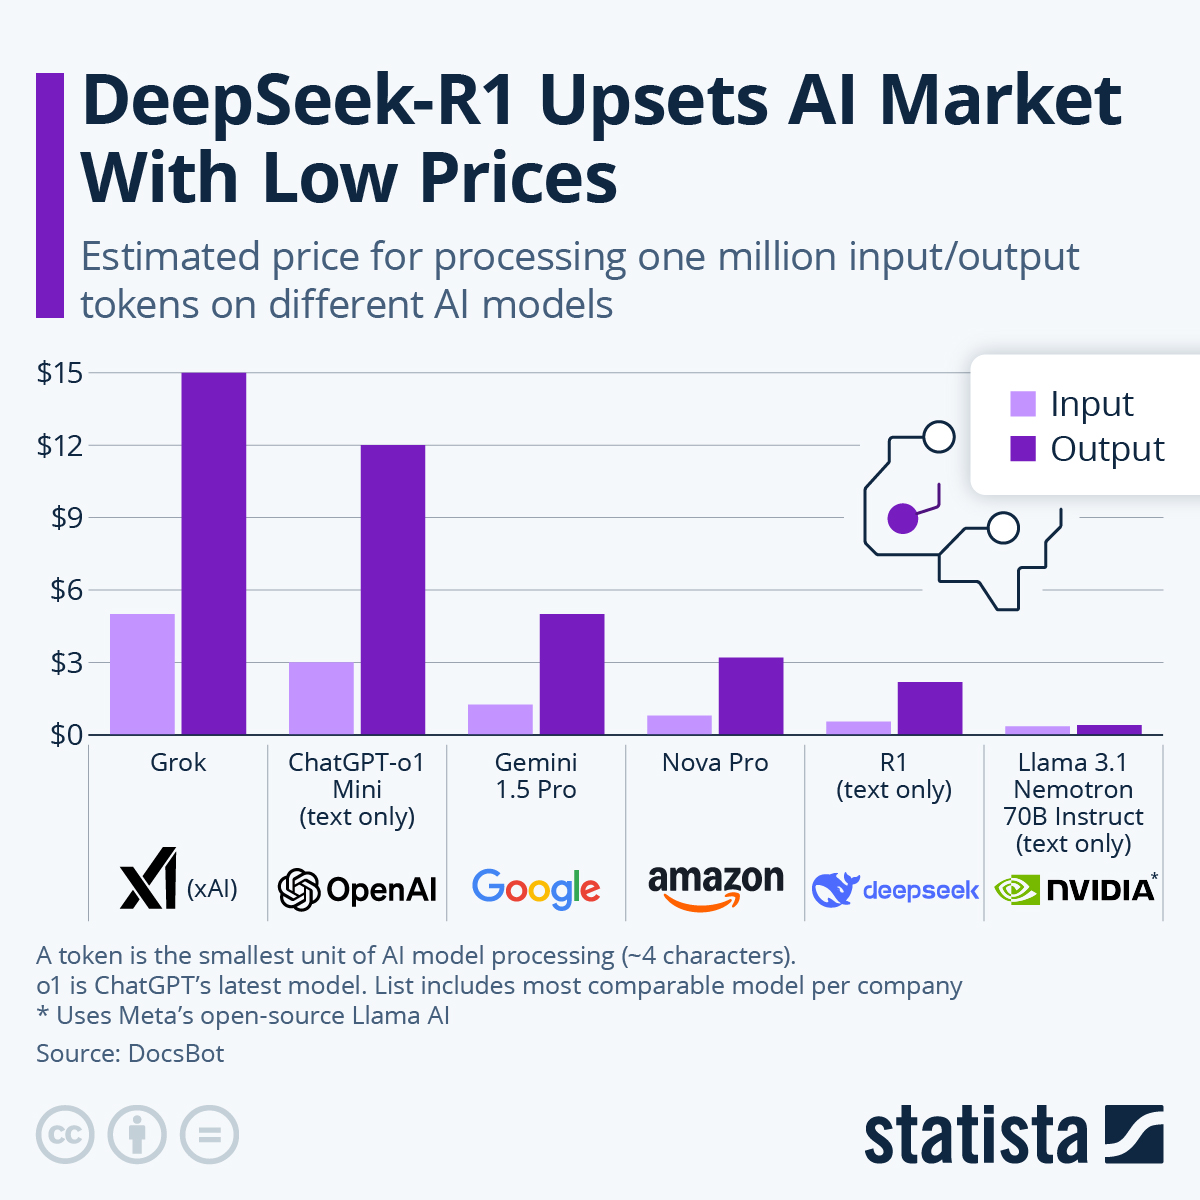
\includegraphics[width=0.8\textwidth]{img/deepseekr1_vs_openaio1.jpeg}
    \caption{Comparison of input and output token pricing across AI models. Source: \cite{buchholz2025deepseekprices}.}
    \label{fig:deepseekr1_vs_openaio1}
\end{figure}


\section{Historical Data}
\label{sec:historical_data}

The \textbf{Similarweb ``Gen AI Market Winners''} article utilizes \textbf{web traffic and engagement analytics} aggregated by Similarweb \cite{similarweb2026genAIwinners}, (\href{https://www.similarweb.com/blog/insights/marketing-insights/gen-ai-market-winners/}{hyperlink}). The dataset primarily consists of monthly website traffic estimates, supplemented by market share comparisons among leading generative AI platforms. Crucially, this data represents behavioral usage at the web and application levels rather than internal proprietary metrics, such as total tokens processed. Nevertheless, it serves as a reliable proxy for user demand, making it a suitable dataset for analyzing adoption trends and competitive positioning within the generative AI market.

\noindent \textbf{Scope: Global.} The traffic series is treated as a global adoption proxy, as the Similarweb report provides overall platform visit estimates without applying specific geographic filters for this analysis \cite{similarweb2026genAIwinners}.

\section{Estimating the Bass Model}
\label{sec:bass_model}

The Bass diffusion model describes adoption driven by three primary factors:
\begin{enumerate}
    \item \textbf{Innovation} ($p$): The likelihood of adoption due to external influence (advertising, news).
    \item \textbf{Imitation} ($q$): The likelihood of adoption due to internal influence (word-of-mouth).
    \item \textbf{Market Potential} ($M$): The total number of potential adopters in the market.
\end{enumerate}

Let $A(t)$ be the cumulative number of adopters by time $t$, and $a(t)$ be the number of adopters in period $t$. Consequently, the cumulative and individual rates of adoption are defined as $F(t) = \frac{A(t)}{M}$ and $f(t) = \frac{a(t)}{M}$, respectively.

Solving the Bass model differential equation yields the cumulative distribution function:
$$
F(t) = \frac{1 - e^{-(p+q)t}}{1 + \frac{q}{p} e^{-(p+q)t}}.
$$

Given the discrete nature of the data, we model the number of adopters in period $t$, denoted as $\hat{a}_t$, as follows:
$$
\hat{a}_t = \hat{A}(t) - \hat{A}(t-1) = M \left( F(t) - F(t-1) \right).
$$

I estimate the parameters $M, p,$ and $q$ by minimizing the Sum of Squared Errors (SSE) between the observed monthly adopters and the Bass model predictions:
$$
\arg \min_{M,p,q} \sum_{t=1}^T \left( a_t - \hat{a}_t(M,p,q) \right)^2.
$$

The quality of the model fit is evaluated using the Root Mean Square Error (RMSE).

\subsubsection{Fitted Models}
\label{subsubsec:fitted_models}

\textbf{DeepSeek:} $\quad \hat{M} = 7287.40, \quad \hat{p} = 0.06143, \quad \hat{q} = 0.07428.$

\noindent \textbf{OpenAI:} $\quad \hat{M} = 111177.74, \quad \hat{p} = 0.03195, \quad \hat{q} = 0.14453.$

\noindent Here, $\hat{M}$ represents the market potential in millions of cumulative visits. For DeepSeek, $\hat{p}$ is relatively close to $\hat{q}$, suggesting that adoption was driven by both significant external interest and subsequent word-of-mouth. For the OpenAI (ChatGPT) proxy, $\hat{p}$ is notably lower than $\hat{q}$, indicating that growth is primarily driven by imitation and widespread social diffusion, consistent with prior observations \cite{microsoft2025globalAI}.

While the classical Bass model assumes a smooth diffusion path, web traffic data often exhibits spikes due to exogenous events. This volatility can increase the error for series with sharp fluctuations. Nevertheless, the Bass model provides a robust first-order summary of diffusion and serves as a reliable basis for forecasting.

\subsubsection{Look-alike Parameter Transfer}
\label{subsubsec:parameter_transfer}
A parameter transfer experiment is also conducted. This involves adopting the innovation ($p$) and imitation ($q$) coefficients from the look-alike innovation (OpenAI) and re-estimating only the market potential ($M$) for DeepSeek to predict its adoption rate, $\hat{a}_t$.

\section{Diffusion Model Analysis}
\label{sec:diffusion_analysis}

\begin{figure}[h]
\centering
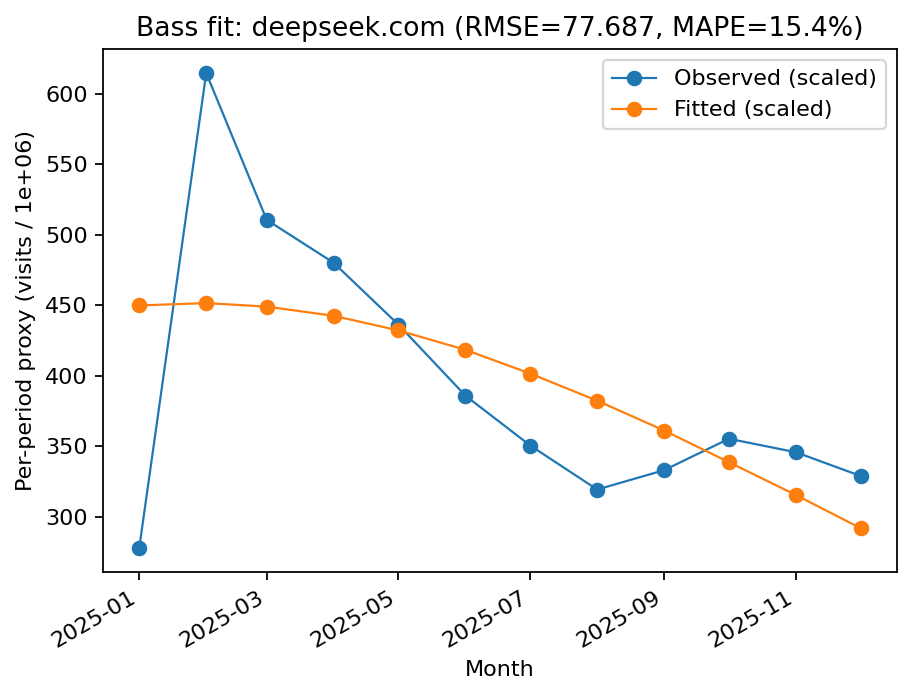
\includegraphics[width=0.48\textwidth]{img/bass2025_deepseek_com_fit.png}
\hfill
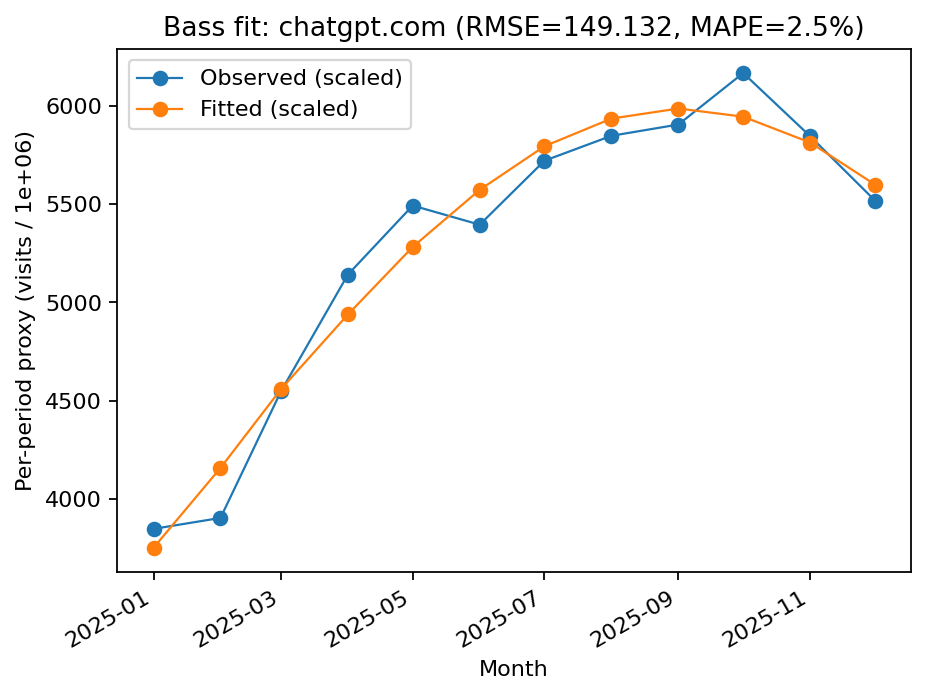
\includegraphics[width=0.48\textwidth]{img/bass2025_chatgpt_com_fit.png}
\caption{Monthly adoption proxy $a_t$ (observed) and Bass fitted $\hat{a}_t$ (millions of visits).}
\label{fig:period_fit}
\end{figure}

\begin{figure}[h]
\centering
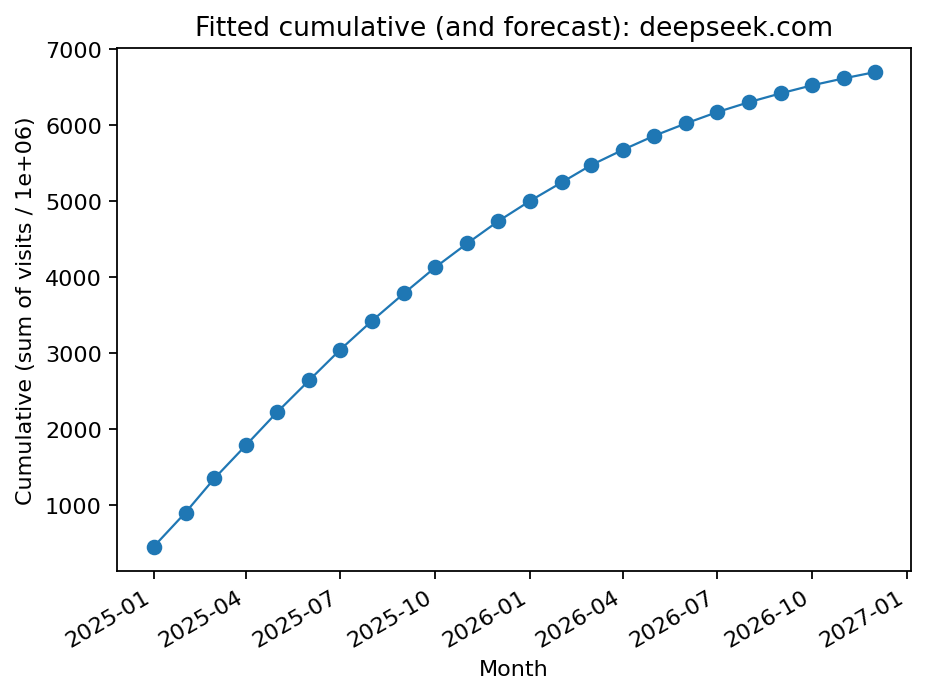
\includegraphics[width=0.48\textwidth]{img/bass2025_deepseek_com_cumulative.png}
\hfill
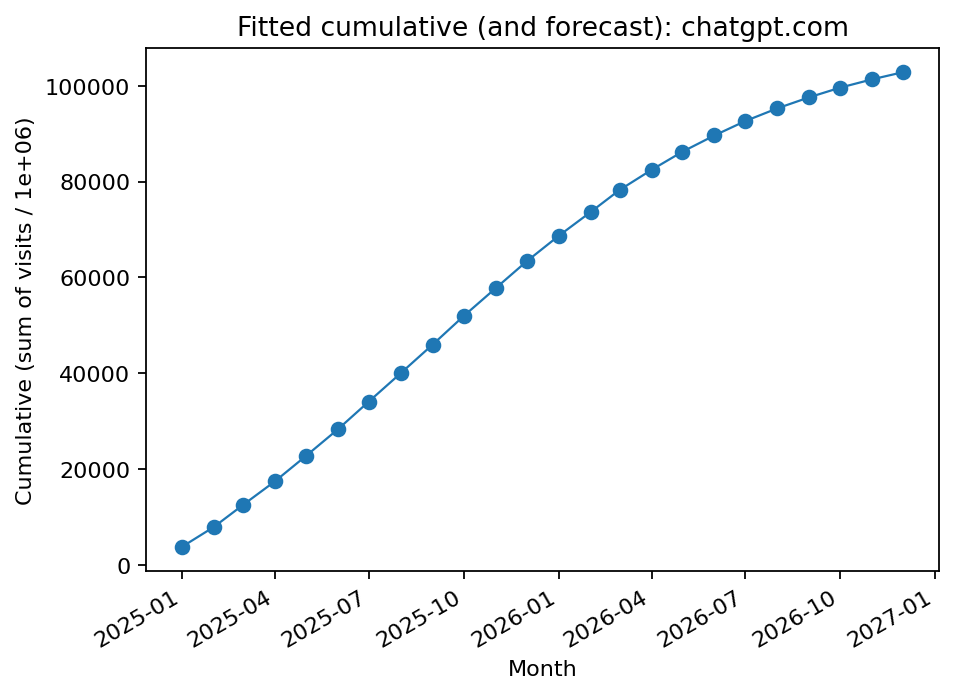
\includegraphics[width=0.48\textwidth]{img/bass2025_chatgpt_com_cumulative.png}
\caption{Cumulative Bass diffusion paths $\hat{A}(t)$ implied by the fitted models (millions of visits).}
\label{fig:cumulative_fit}
\end{figure}

\begin{figure}[h]
\centering
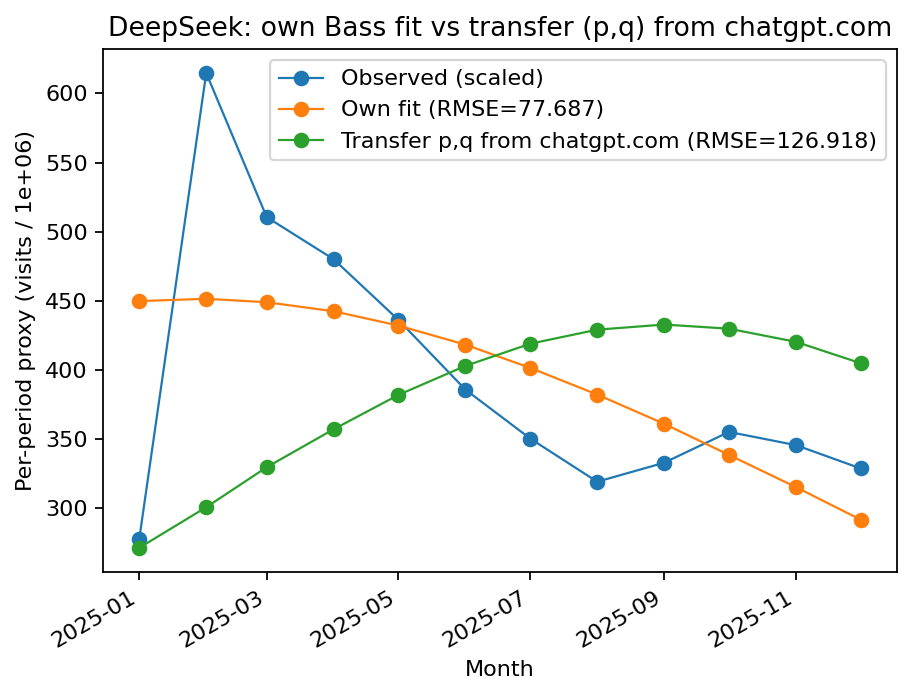
\includegraphics[width=0.96\textwidth]{img/bass2025_deepseek_com_transfer_from_chatgpt_com_fit.png}
\caption{DeepSeek monthly adoption proxy $a_t$ (observed) compared against: (i) DeepSeek's own fitted Bass model and (ii) a transfer model that reuses coefficients $(\hat{p}, \hat{q})$ from chatgpt.com while re-estimating $M$ for DeepSeek. The transfer model exhibits higher error (RMSE), suggesting that DeepSeek's diffusion dynamics are distinct from those of GPT-o1.}
\label{fig:deepseek_transfer_fit}
\end{figure}

Exact monthly values and model outputs are reported in Appendix~\ref{app:tables}, specifically in Tables~\ref{tab:deepseek_own_values} and \ref{tab:deepseek_transfer_values}.

\newpage

\section{Conclusion}
\label{sec:conclusion}

\subsection{Limitations}
\label{subsec:limitations}

This study is subject to several limitations that should be noted. First, external factors such as sovereign AI usage tendencies and national safe-usage regulations were not considered due to the inherent ambiguity of these phenomena and the inability to provide exact measures or decay effects. Second, the broader impact on the AI hardware market, including key players such as NVIDIA, was not analyzed. Furthermore, while industry allegations have surfaced regarding DeepSeek's data collection methods in relation to OpenAI, these claims remain unproven and were therefore excluded to maintain the factual integrity of the study.

Another limitation involves the primary data source. While Similarweb provides a robust overview of the general market, access to a wider variety of data sources could lead to more precise estimates. Other data providers, such as \href{https://openrouter.ai/deepseek/deepseek-r1:free}{OpenRouter} and Statista (\href{https://www.statista.com/statistics/1561128/deepseek-daily-active-users/?srsltid=AfmBOoropm3jOgkgdZMGQ9fweLhZLJK4jN3-YnUfzRHfzdQ_QObnmRie}{Source 1}, \href{https://www.statista.com/statistics/1659718/global-monthly-chatgpt-users/?srsltid=AfmBOor9vFsVYNFJTC6oLSHMlqm6DtZzO4DCZNnO8TtU1KTyhnIJoj2l}{Source 2}), provide alternative perspectives on daily and monthly usage; however, these were not utilized in the current analysis due to paywall constraints. Finally, the acquisition of high-frequency or "smoother" data would likely improve the convergence and overall fit of the Bass diffusion model.

\appendix
\section{Appendix: Monthly adoption tables}
\label{app:tables}

\subsection{OpenAI monthly table (own fit)}
\scriptsize
\begin{longtable}{lrrr}
\caption{OpenAI (chatgpt.com) monthly adoption proxy and Bass own-fit (millions of visits). Observed values are not available for forecast months.} \label{tab:openai_own_values} \\
\toprule
month & Observed $a_t$ & Fitted $\hat{a}_t$ & Fitted $\hat{A}(t)$ \\
\midrule
\endfirsthead
\caption[]{OpenAI (chatgpt.com) monthly adoption proxy and Bass own-fit (millions of visits). Observed values are not available for forecast months.} \\
\toprule
month & Observed $a_t$ & Fitted $\hat{a}_t$ & Fitted $\hat{A}(t)$ \\
\midrule
\endhead
\midrule
\multicolumn{4}{r}{Continued on next page} \\
\midrule
\endfoot
\bottomrule
\endlastfoot
2025-01 & 3849.850000 & 3753.640000 & 3753.640000 \\
2025-02 & 3905.400000 & 4159.380000 & 7913.020000 \\
2025-03 & 4548.610000 & 4559.430000 & 12472.450000 \\
2025-04 & 5141.780000 & 4939.090000 & 17411.540000 \\
2025-05 & 5492.390000 & 5282.190000 & 22693.730000 \\
2025-06 & 5395.130000 & 5572.190000 & 28265.920000 \\
2025-07 & 5720.230000 & 5793.750000 & 34059.670000 \\
2025-08 & 5846.790000 & 5934.270000 & 39993.940000 \\
2025-09 & 5904.120000 & 5985.360000 & 45979.300000 \\
2025-10 & 6165.610000 & 5943.920000 & 51923.220000 \\
2025-11 & 5844.550000 & 5812.480000 & 57735.700000 \\
2025-12 & 5517.990000 & 5598.890000 & 63334.590000 \\
2026-01 & -- & 5315.380000 & 68649.970000 \\
2026-02 & -- & 4977.080000 & 73627.050000 \\
2026-03 & -- & 4600.470000 & 78227.520000 \\
2026-04 & -- & 4201.850000 & 82429.370000 \\
2026-05 & -- & 3796.080000 & 86225.440000 \\
2026-06 & -- & 3395.800000 & 89621.240000 \\
2026-07 & -- & 3011.010000 & 92632.250000 \\
2026-08 & -- & 2648.980000 & 95281.230000 \\
2026-09 & -- & 2314.450000 & 97595.680000 \\
2026-10 & -- & 2010.010000 & 99605.690000 \\
2026-11 & -- & 1736.500000 & 101342.190000 \\
2026-12 & -- & 1493.420000 & 102835.610000 \\
\end{longtable}

\normalsize

\subsection{DeepSeek monthly table (own fit)}
\scriptsize
\begin{longtable}{lrrr}
\caption{DeepSeek (deepseek.com) monthly adoption proxy and Bass own-fit (millions of visits). Observed values are not available for forecast months.} \label{tab:deepseek_own_values} \\
\toprule
month & Observed $a_t$ & Fitted $\hat{a}_t$ & Fitted $\hat{A}(t)$ \\
\midrule
\endfirsthead
\caption[]{DeepSeek (deepseek.com) monthly adoption proxy and Bass own-fit (millions of visits). Observed values are not available for forecast months.} \\
\toprule
month & Observed $a_t$ & Fitted $\hat{a}_t$ & Fitted $\hat{A}(t)$ \\
\midrule
\endhead
\midrule
\multicolumn{4}{r}{Continued on next page} \\
\midrule
\endfoot
\bottomrule
\endlastfoot
2025-01 & 277.910000 & 449.870000 & 449.870000 \\
2025-02 & 614.740000 & 451.530000 & 901.400000 \\
2025-03 & 510.560000 & 449.040000 & 1350.440000 \\
2025-04 & 480.120000 & 442.510000 & 1792.950000 \\
2025-05 & 436.200000 & 432.160000 & 2225.110000 \\
2025-06 & 385.850000 & 418.360000 & 2643.470000 \\
2025-07 & 350.480000 & 401.560000 & 3045.030000 \\
2025-08 & 319.270000 & 382.300000 & 3427.320000 \\
2025-09 & 333.000000 & 361.130000 & 3788.450000 \\
2025-10 & 355.280000 & 338.640000 & 4127.100000 \\
2025-11 & 345.710000 & 315.370000 & 4442.460000 \\
2025-12 & 328.870000 & 291.810000 & 4734.270000 \\
2026-01 & -- & 268.410000 & 5002.680000 \\
2026-02 & -- & 245.540000 & 5248.220000 \\
2026-03 & -- & 223.500000 & 5471.720000 \\
2026-04 & -- & 202.510000 & 5674.220000 \\
2026-05 & -- & 182.730000 & 5856.950000 \\
2026-06 & -- & 164.270000 & 6021.220000 \\
2026-07 & -- & 147.180000 & 6168.400000 \\
2026-08 & -- & 131.480000 & 6299.880000 \\
2026-09 & -- & 117.130000 & 6417.010000 \\
2026-10 & -- & 104.100000 & 6521.110000 \\
2026-11 & -- & 92.330000 & 6613.440000 \\
2026-12 & -- & 81.730000 & 6695.160000 \\
\end{longtable}

\normalsize

\subsection{DeepSeek monthly table (transfer from chatgpt.com)}
\scriptsize
\begin{longtable}{lrrr}
\caption{DeepSeek monthly adoption proxy and Bass transfer fit (millions of visits). Transfer model reuses $(\hat p,\hat q)$ from chatgpt.com and re-estimates $M$ for DeepSeek. Observed values are not available for forecast months.} \label{tab:deepseek_transfer_values} \\
\toprule
month & Observed $a_t$ & Transfer $\hat{a}_t$ & Transfer $\hat{A}(t)$ \\
\midrule
\endfirsthead
\caption[]{DeepSeek monthly adoption proxy and Bass transfer fit (millions of visits). Transfer model reuses $(\hat p,\hat q)$ from chatgpt.com and re-estimates $M$ for DeepSeek. Observed values are not available for forecast months.} \\
\toprule
month & Observed $a_t$ & Transfer $\hat{a}_t$ & Transfer $\hat{A}(t)$ \\
\midrule
\endhead
\midrule
\multicolumn{4}{r}{Continued on next page} \\
\midrule
\endfoot
\bottomrule
\endlastfoot
2025-01 & 277.910000 & 271.490000 & 271.490000 \\
2025-02 & 614.740000 & 300.840000 & 572.330000 \\
2025-03 & 510.560000 & 329.770000 & 902.100000 \\
2025-04 & 480.120000 & 357.230000 & 1259.330000 \\
2025-05 & 436.200000 & 382.050000 & 1641.380000 \\
2025-06 & 385.850000 & 403.020000 & 2044.400000 \\
2025-07 & 350.480000 & 419.050000 & 2463.440000 \\
2025-08 & 319.270000 & 429.210000 & 2892.650000 \\
2025-09 & 333.000000 & 432.900000 & 3325.560000 \\
2025-10 & 355.280000 & 429.910000 & 3755.460000 \\
2025-11 & 345.710000 & 420.400000 & 4175.860000 \\
2025-12 & 328.870000 & 404.950000 & 4580.820000 \\
2026-01 & -- & 384.450000 & 4965.260000 \\
2026-02 & -- & 359.980000 & 5325.240000 \\
2026-03 & -- & 332.740000 & 5657.980000 \\
2026-04 & -- & 303.910000 & 5961.890000 \\
2026-05 & -- & 274.560000 & 6236.450000 \\
2026-06 & -- & 245.610000 & 6482.060000 \\
2026-07 & -- & 217.780000 & 6699.840000 \\
2026-08 & -- & 191.590000 & 6891.430000 \\
2026-09 & -- & 167.400000 & 7058.830000 \\
2026-10 & -- & 145.380000 & 7204.210000 \\
2026-11 & -- & 125.600000 & 7329.800000 \\
2026-12 & -- & 108.020000 & 7437.820000 \\
\end{longtable}

\normalsize

\newpage
\bibliographystyle{plain} % Or 'unsrt', 'alpha', etc.
\bibliography{references}  % This must match your filename 'references.bib'

\end{document}